
\begin{frame}{L'IA est complexe !}
  \begin{center}
    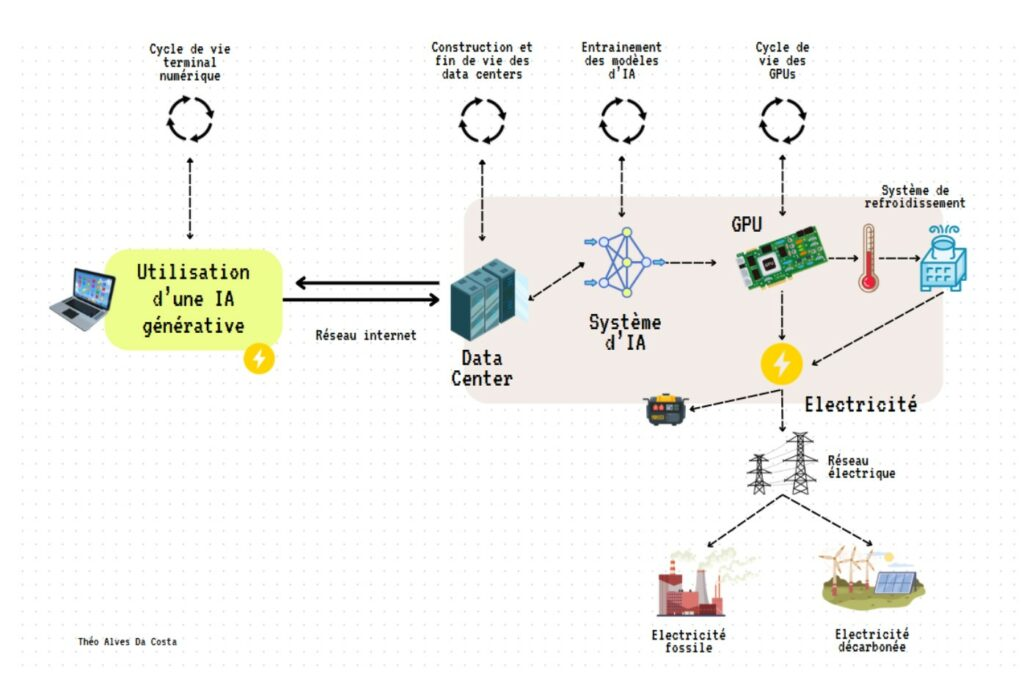
\includegraphics[width=\textwidth]{img/intro/IMAGE-6-credit-Bon-Pote-Theo-Alves-Da-costa-article-IA-1024x682.jpg}
  \end{center}

  {\footnotesize
  Ref : \href{https://bonpote.com/intelligence-artificielle-le-vrai-cout-environnemental-de-la-course-a-lia/}{\underline{Intelligence artificielle : le vrai coût environnemental de la course à l'IA}}}

\end{frame}

\section{Empreinte Carbone de l'IA}

\begin{frame}{Coût environnemental de l'IA générative}

\textbf{L'essor de l'IA générative}
\begin{itemize}
    \item Depuis 2022, adoption massive de l'IA générative (ChatGPT)
    \item Croissance bien plus rapide que les réseaux sociaux
    \item Repose sur des \textbf{LLM} entraînés sur d'énormes quantités de données
    \item Techniques : deep learning et transformers
    \item Modèles \textcolor{red}{10 000 fois plus gros} qu'en 2018
\end{itemize}

\end{frame}

\begin{frame}{Trois facteurs aggravants}

\begin{enumerate}
    \item<+-> \textbf{Croissance exponentielle de l'usage}
        \begin{itemize}
            \item Des millions d'utilisateurs quotidiens
            \item 40\% des ménages aux États-Unis/Royaume-Uni
            \item Plus de 50\% dans certains pays en développement
        \end{itemize}

    \vspace{0.2cm}
    \item<+-> \textbf{Complexification des modèles}
        \begin{itemize}
            \item Modèles plus gros
            \item Plus gourmands en données et en puissance de calcul
        \end{itemize}

    \vspace{0.2cm}
    \item<+-> \textbf{Développement des data centers}
        \begin{itemize}
            \item Accélération de la construction d'infrastructures énergivores
            \item Impacts locaux : électricité, eau, pollution
        \end{itemize}
\end{enumerate}

\end{frame}

\begin{frame}{Processus énergivore : Entraînement}

\textbf{L'entraînement des modèles :}

\vspace{0.3cm}

\begin{itemize}
    \item Nécessite des milliers de GPU (ex. : H100 de Nvidia) en parallèle
    \item Les émissions varient selon la taille du modèle et l'intensité carbone
\end{itemize}

\vspace{0.5cm}

\onslide<2>
\textbf{Exemple : Llama 3.1 (405B paramètres)}
\begin{itemize}
    \item Consommation : \textcolor{red}{8,6 GWh}
    \item Équivalent à \textcolor{red}{4 500 années de calcul} sur un seul GPU
\end{itemize}

\end{frame}

\begin{frame}{Processus énergivore : Inférence}

\textbf{L'inférence (usage quotidien) :}

\vspace{0.3cm}

\begin{itemize}
    \item<+-> Aujourd'hui, \textcolor{red}{l'usage dépasse largement le coût de l'entraînement}
        \begin{itemize}
            \item Seuil atteint après ~100 millions d'utilisations
        \end{itemize}

    \vspace{0.2cm}
    \item<+-> Une requête ChatGPT peut consommer autant qu'une recherche Google
        \begin{itemize}
            \item Mais les données manquent pour le confirmer
        \end{itemize}

    \vspace{0.2cm}
    \item<+-> \textbf{Tâches les plus énergivores :}
        \begin{itemize}
            \item Génération de vidéos : \textcolor{red}{115 Wh} pour 6 secondes
            \item Génération d'images : 1-3 Wh
            \item Génération de texte : 0,3 Wh
        \end{itemize}
\end{itemize}

\end{frame}

\begin{frame}{Problème de transparence}

\begin{columns}
\begin{column}{0.48\textwidth}
    \colorwarning{red}\textbf{Manque de données fiables :}
    \begin{itemize}
        \item Les géants de l'IA ne communiquent presque rien
        \item OpenAI, Meta, etc. : opacité totale
        \item Seulement \textcolor{red}{2\% des usages} concernent des modèles transparents (ex : Llama 3.3)
    \end{itemize}
\end{column}

\begin{column}{0.48\textwidth}
    \onslide<2>
    \colorwarning{red}\textbf{Chiffres contestés :}
    \begin{itemize}
        \item Affirmation : "1 requête ChatGPT = 10 recherches Google"
        \item Mal documentée et datée
        \item Manque de vérification
    \end{itemize}
\end{column}
\end{columns}

\vspace{0.5cm}

\textbf{Problème clé :} Impossible d'évaluer précisément l'impact sans transparence

\end{frame}

\begin{frame}{Enjeux plus larges}

\textbf{L'IA n'est pas neutre :}

\vspace{0.3cm}

\begin{itemize}
    \item<+-> \textbf{Biais et données}
        \begin{itemize}
            \item Reproduit des biais existants
            \item Dépend de données souvent extraites sans consentement
        \end{itemize}

    \vspace{0.2cm}
    \item<+-> \textbf{Impact géopolitique et industriel}
        \begin{itemize}
            \item Enjeu économique et stratégique majeur
            \item Conséquences environnementales sous-estimées
        \end{itemize}
\end{itemize}

\vspace{0.5cm}
\onslide<2>
\textbf{Conclusion :} Besoin urgent de régulation et de mesures d'impact

\end{frame}

\begin{frame}{Conclusion : Coût environnemental croissant}

\textbf{Points clés :}

\vspace{0.3cm}

\begin{itemize}
    \item L'IA générative a un \textcolor{red}{coût environnemental croissant}
    \item Dominé par l'usage quotidien plutôt que l'entraînement
    \item Manque de transparence empêche une évaluation précise
    \item Projections : \textcolor{red}{demande énergétique en hausse}
    \item Surtout avec génération multimédia (vidéo, image)
\end{itemize}

\vspace{0.5cm}

\textbf{Urgence :} Régulation et mesures d'impact transparentes

\vspace{0.3cm}

\small{(Sources : Epoch AI, MIT, Sasha Luccioni, rapports sectoriels)}

\end{frame}

\begin{frame}
\frametitle{Optimisation de la consommation électrique}
\framesubtitle{Techniques et limites}

\textbf{L'industrie développe des solutions :}

\vspace{0.3cm}

\begin{itemize}
    \item<+-> \textbf{Optimisations logicielles}
        \begin{itemize}
            \item Quantification : réduire la précision des données
            \item Élagage (pruning) : supprimer les parties inutiles
            \item Distillation : créer des versions allégées
            \item Architecture MoE : utiliser seulement une partie du modèle
        \end{itemize}

    \vspace{0.2cm}
    \item<+-> \textbf{Optimisations de déploiement}
        \begin{itemize}
            \item Batch inference : traiter plusieurs demandes simultanément
            \item Compilateurs spécialisés : éviter les redondances
        \end{itemize}
\end{itemize}

\end{frame}

\begin{frame}{Optimisations matérielles}

\textbf{Optimisations matérielles et infrastructuelles :}

\vspace{0.3cm}

\begin{itemize}
    \item<+-> \textbf{Puces spécialisées}
        \begin{itemize}
            \item TPUs, LPUs plus écoénergétiques que GPU classiques
        \end{itemize}

    \vspace{0.2cm}
    \item<+-> \textbf{Amélioration du PUE}
        \begin{itemize}
            \item PUE = Power Usage Effectiveness
            \item Refroidissement optimisé
            \item Gestion en temps réel
        \end{itemize}

    \vspace{0.2cm}
    \item<+-> \textbf{Modèles légers (SLMs)}
        \begin{itemize}
            \item Théoriquement moins gourmands
            \item Mais risque d'\textcolor{red}{augmenter la demande globale}
            \item Ex : assistants IA intégrés dans smartphones
        \end{itemize}
\end{itemize}

\end{frame}

\begin{frame}{Limites des optimisations : L'effet rebond}

\textbf{Malgré les avancées, la consommation totale augmente :}

\vspace{0.3cm}

\begin{itemize}
    \item<+-> \textbf{Effets rebonds directs}
        \begin{itemize}
            \item L'efficacité réduit le coût par requête
            \item Mais \textcolor{red}{stimule une adoption plus massive}
            \item NVIDIA : \textcolor{red}{3,7 millions de GPU vendus en 2024} (+1M vs 2023)
            \item Data centers plus nombreux et plus énergivores
        \end{itemize}

    \vspace{0.2cm}
    \item<+-> \textbf{Effets rebonds indirects}
        \begin{itemize}
            \item L'IA intégrée dans d'autres secteurs polluants
            \item Finance, logistique, etc.
            \item Nouveaux produits manufacturés (puces GPU)
            \item Accélération de l'obsolescence
        \end{itemize}
\end{itemize}

\end{frame}

\begin{frame}{Cas emblématique : DeepSeek-R1}

\textbf{Le piège du "chain-of-thought"}

\vspace{0.3cm}

\begin{itemize}
    \item<+-> \textbf{Prétention médiatique}
        \begin{itemize}
            \item Présenté comme une révolution énergétique
        \end{itemize}

    \vspace{0.2cm}
    \item<+-> \textbf{Réalité}
        \begin{itemize}
            \item Utilise des techniques d'optimisation (MoE)
            \item Mais \textcolor{red}{compense par surconsommation à l'usage}
            \item Méthode "chain-of-thought" : raisonnement étendu
            \item Réponses \textcolor{red}{4,4 fois plus longues}
            \item Consommation : \textcolor{red}{+87\% en moyenne}
            \item Jusqu'à \textcolor{red}{+97x} dans certains cas
        \end{itemize}

    \vspace{0.2cm}
    \item<+-> \textbf{Avertissement des chercheurs}
        \begin{itemize}
            \item Si cette approche se généralise
            \item L'empreinte énergétique de l'inférence \textcolor{red}{exploserait}
        \end{itemize}
\end{itemize}

\end{frame}

\begin{frame}{Conclusion : Un déséquilibre persistant}

\textbf{Constats :}

\vspace{0.3cm}

\begin{itemize}
    \item La puissance de calcul nécessaire \textcolor{red}{double tous les 6 mois}
    \item Les optimisations sont \textcolor{red}{contrecarrées} par :
        \begin{itemize}
            \item Croissance exponentielle des usages
            \item Multiplication des infrastructures
        \end{itemize}
\end{itemize}

\vspace{0.5cm}

\textbf{Solutions urgentes :}
\begin{itemize}
    \item Régulation
    \item Transparence sur l'impact réel (pas seulement théorique)
    \item Évitement des effets rebonds
\end{itemize}

\vspace{0.3cm}

\small{(Sources : Luccioni et al. 2025, MIT Technology Review, rapports sectoriels)}

\end{frame}
